% -*- mode: latex; -*- mustache tags:  
\documentclass[10pt,twoside,english]{_support/latex/sbabook/sbabook}
\let\wholebook=\relax

\usepackage{import}
\subimport{_support/latex/}{common.tex}

%=================================================================
% Debug packages for page layout and overfull lines
% Remove the showtrims document option before printing
\ifshowtrims
  \usepackage{showframe}
  \usepackage[color=magenta,width=5mm]{_support/latex/overcolored}
\fi


% =================================================================
\title{A PharoThings Tutorial}
\author{Allex Oliveira}
\series{Square Bracket tutorials}

\hypersetup{
  pdftitle = {A PharoThings Tutorial},
  pdfauthor = {Allex Oliveira},
  pdfkeywords = {IoT, Raspberry, PharoThings, Pharo}
}


% =================================================================
\begin{document}

% Title page and colophon on verso
\maketitle
\pagestyle{titlingpage}
\thispagestyle{titlingpage} % \pagestyle does not work on the first one…

\cleartoverso
{\small

  Copyright 2017 by Allex Oliveira.

  The contents of this book are protected under the Creative Commons
  Attribution-ShareAlike 3.0 Unported license.

  You are \textbf{free}:
  \begin{itemize}
  \item to \textbf{Share}: to copy, distribute and transmit the work,
  \item to \textbf{Remix}: to adapt the work,
  \end{itemize}

  Under the following conditions:
  \begin{description}
  \item[Attribution.] You must attribute the work in the manner specified by the
    author or licensor (but not in any way that suggests that they endorse you
    or your use of the work).
  \item[Share Alike.] If you alter, transform, or build upon this work, you may
    distribute the resulting work only under the same, similar or a compatible
    license.
  \end{description}

  For any reuse or distribution, you must make clear to others the
  license terms of this work. The best way to do this is with a link to
  this web page: \\
  \url{http://creativecommons.org/licenses/by-sa/3.0/}

  Any of the above conditions can be waived if you get permission from
  the copyright holder. Nothing in this license impairs or restricts the
  author's moral rights.

  \begin{center}
    
\includegraphics[width=0.2\textwidth]{_support/latex/sbabook/CreativeCommons-BY-SA.pdf}
  \end{center}

  Your fair dealing and other rights are in no way affected by the
  above. This is a human-readable summary of the Legal Code (the full
  license): \\
  \url{http://creativecommons.org/licenses/by-sa/3.0/legalcode}

  \vfill

  % Publication info would go here (publisher, ISBN, cover design…)
  Layout and typography based on the \textcode{sbabook} \LaTeX{} class by Damien
  Pollet.
}


\frontmatter
\pagestyle{plain}

\tableofcontents*
\clearpage\listoffigures

\mainmatter

\chapter{Lesson 8 - I2C Sensors (Temperature, Humidity, Pressure and Acellerometer)}
In the previous lessons, we learned how to control LEDs and to use a button to interact with LEDs. Now let's start using some sensors to interact automatically with the real world, taking the temperature, air pressure and humidity This kind of sensor use the I2C protocol to communicate.
\section{What we need?}
In this lesson we will use a setup with 3 different I2C sensors.
\subsection{Components}
\begin{itemize}
\item 1 Raspberry Pi connected to your network (wired or wireless)
\item 1 Breadboard
\item 1 BME280 temperature, humidity and pressure sensor
\item 1 MCP9808 temperature sensor
\item 1 ADXL345 accelerometer sensor
\item Jumper wires
\end{itemize}
\section{Experimental theory}
Before constructing any circuit, you must know the parameters of the components in the circuit, such as their operating voltage, operating circuit, etc.
\subsection{The I2C protocol}
The I2C communication protocol can be easily implemented in many electronic projects, being a very popular and widely used protocol. It is possible to perform communication between one or more master devices and several slave devices. It is an easy-to-implement protocol because it uses only 2 wires to communicate between up to 112 devices using 7-bit addressing and up to 1008 devices using 10-bit addressing.

The Figure \ref{I2CBus} shows how you can connect the devices using the same I2C bus.


\begin{figure}

\begin{center}
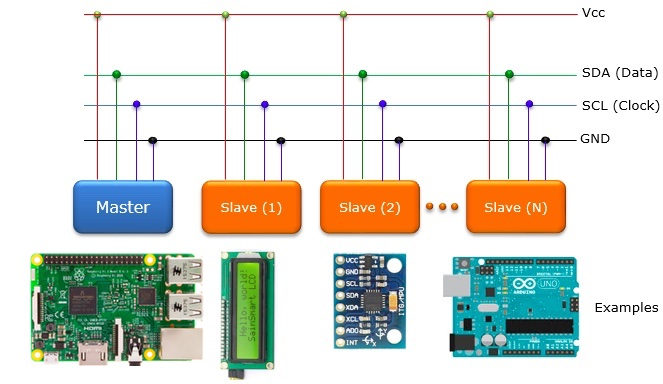
\includegraphics[width=0.8\textwidth]{/Users/allexoliveira/PharoThingsBook/Booklet-APharoThingTutorial/_result/pdf/Chapters/Chap9I2CSensors/figures/pharothings-i2c-bus.jpg}\caption{Devices connected using I2C bus.\label{I2CBus}}\end{center}
\end{figure}

\subsection{How I2C works?}
How can we communicate with multiple devices using only two wires? For this to happen, each device has set an ID or an unique address. Then the master device can choose which device to communicate with.

The two wires are called Serial Clock (or SCL) and Serial Data (or SDA). The SCL wire is the clock signal that synchronizes the data transfer between devices on the I2C bus and is generated by the master device. The other wire is the SDA line that carries the date.
\subsection{Protocol}
The data is transferred in 8-bit sequences, like you can see in Figure \ref{I2CBusPacket}. After a special starting condition occurs, comes the first 8-bit sequence that indicates the address of the slave to which the data is being sent.
For example, for the ADXL345 accelerometer device, the default address is 16r53 (0X53) or 0101 0011 (the last bit actived means the device is on read mode).

After each 8 bit sequence follows a bit called Acknowledge. After the first Acknowledge bit, in most cases another addressing sequence comes, but this time to the internal registers of the slave device. 

The internal registers are locations in the slave's memory containing various information or data. For example, the ADX345 accelerometer has a unique device address (16r53) and addition internal record addresses for the X, Y, and Z axes (16r32, 16r33, 16r34, etc.). Therefore, if we want to read the X-axis data, we first need to send the address of the device and then the internal register address specific to the X-axis.

After the addressing sequences, the data streams are as many as they are sent until the data is completely sent and ends with a special stop condition.


\begin{figure}

\begin{center}
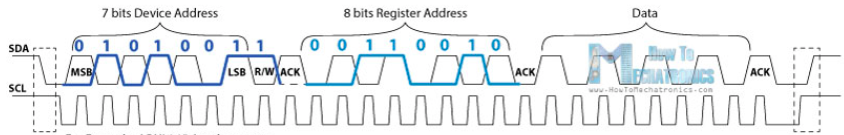
\includegraphics[width=0.8\textwidth]{/Users/allexoliveira/PharoThingsBook/Booklet-APharoThingTutorial/_result/pdf/Chapters/Chap9I2CSensors/figures/pharothings-i2c-bus-data.png}\caption{Bits sequence.\label{I2CBusPacket}}\end{center}
\end{figure}

\section{Experimental procedure}
Now we will build the circuit. This circuit consists of three sensors (BME280, MCP9808, ADXL345) and a power supply (the Rasp).

\begin{itemize}
\item Connect the Ground PIN from Raspberry in the breadboard blue rail (-). In this experiment we will use the PIN6 (Ground);
\item Then connect the 3.3V (PIN1) pin in the red rail (+). 
\item Now let's conect the SCL (PIN5) and SDA (PIN3) wires. Connect them like as shown in the Figure \ref{physicalSensors} ;
\item Now push the sensors in the breadboard;
\item And insert the jumper wires connecting the sensor in the bus, like as shown in the Figure \ref{physicalSensors};
\item Last step is to connect the power 3.3V (+) and ground (-) wires in each sensor.
\end{itemize}

The Figure \ref{physicalSensors} shows how the electric connection is made.


\begin{figure}

\begin{center}
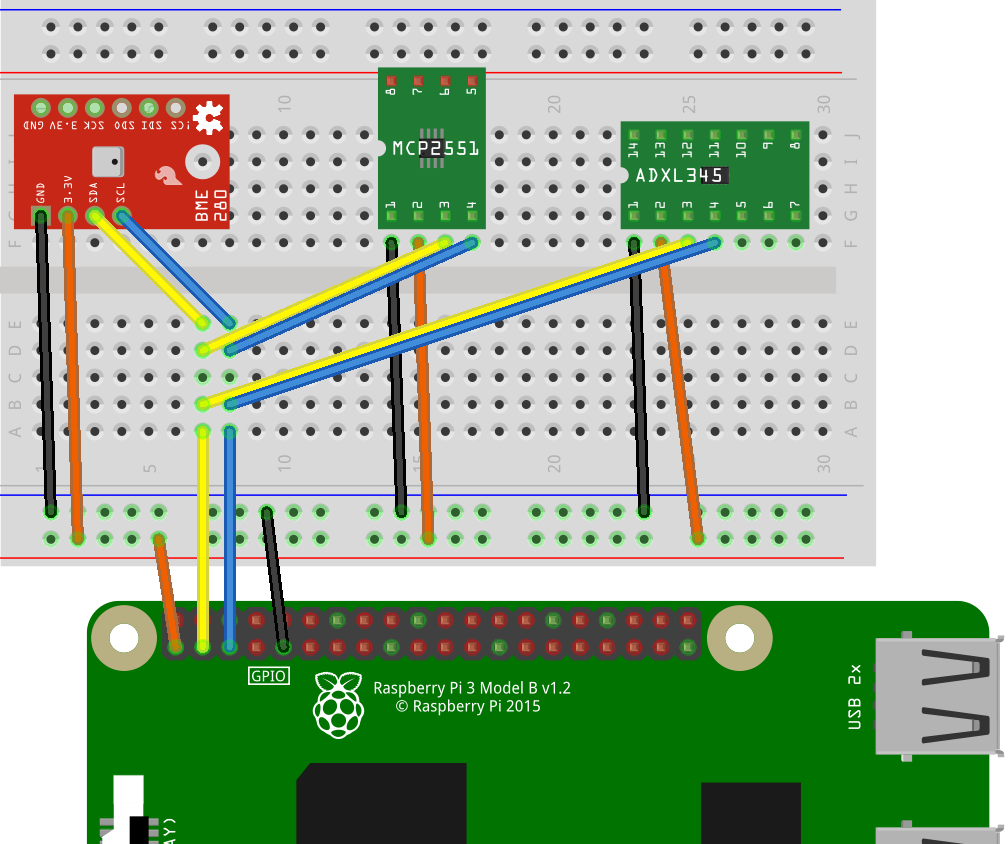
\includegraphics[width=0.6\textwidth]{/Users/allexoliveira/PharoThingsBook/Booklet-APharoThingTutorial/_result/pdf/Chapters/Chap9I2CSensors/figures/pharothings-sensors-board.png}\caption{Physical sensors connection.\label{physicalSensors}}\end{center}
\end{figure}

\section{Configuring the Raspberry Pi I2C}
We need to configure the Raspberrry Pi to use the I2C protocol. To do this, access the Raspberry using SSH and go to file \textcode{/boot/config.txt} and add the line \textcode{dtparam=i2c1=on}.

You can run the follow command to do this:

\begin{displaycode}{plain}
sudo echo dtparam=i2c1=on >> /boot/config.txt
\end{displaycode}

Add the ‘pi’ user to I2C group and restart the Raspberry 

\begin{displaycode}{plain}
sudo adduser pi i2c 
reboot
\end{displaycode}

Now your Raspberry is configured to comunicate with the sensor using the I2C protocol. 
\section{Connecting remotely}
Through your local Pharo image, let’s connect in the Pharo image by running on Raspberry, enable the auto-refresh feature of the inspector, and open the inspector.
Run this code in your local playground:

\begin{displaycode}{plain}
remotePharo := TlpRemoteIDE connectTo: (TCPAddress ip: #[193 51 236 212] port: 40423)
GTInspector enableStepRefresh.
remoteBoard := remotePharo evaluate: [ RpiBoard3B current].
remoteBoard inspect.
\end{displaycode}
\section{Exploring the properties of an remote object with remote inspector}
In your inspect window (Inspector on a PotRemoteBoard), let’s create the instances of the firt sensor. 

\begin{displaycode}{plain}
a := board installDevice: PotBME280Device new. ​
\end{displaycode}

With this procceding we are creating an object and we can inspect it to see the properties and values. To see the details of this object, like for example what you can do and what you can ask to it (methods), press cmd + I to inspect it and you will see the inspect window. 

In the \textcode{Meta} tab, you can see the Class and Subclass of this object. To see what you can do with this object (methods), you can start selecting the top Class and will be show in the right window the methods that you can to use.

Let's see what the method \textcode{readParameters} can do. When you select it, you can see the code of method on bottom of the window. When you call this method, it return an array with 3 values: temperature, pressure and humidity. The carot simbol (little hat ˆ) is to return something when the method is called. 

So let's use the method \textcode{readParameters} to ask to the object what are the values of temperature, pressure and humidity. To get the return of this object, select the follow code and press cmd + P. You will see the a big number. This number is a array with 3 index like the Figure \ref{inspectorSensor}. 


\begin{figure}

\begin{center}
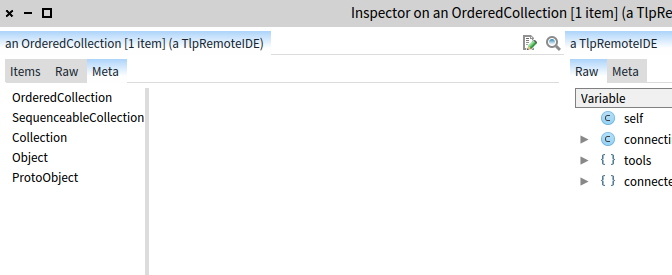
\includegraphics[width=0.8\textwidth]{/Users/allexoliveira/PharoThingsBook/Booklet-APharoThingTutorial/_result/pdf/Chapters/Chap9I2CSensors/figures/pharothings-inspect-sensor.png}\caption{Inspecting remote object.\label{inspectorSensor}}\end{center}
\end{figure}


\begin{displaycode}{plain}
a readParameters.
\end{displaycode}

To see the details of this object, you can press cmd + I to inspect it and you will see the 3 index separately. 
\section{Getting the temperature with BME280}
You can also ask to only one value, selecting the array index using the method \textcode{at:}. In this case we are selecting only the index 1 of array and will return only the temperature:

\begin{displaycode}{plain}
a readParameters at: 1.
\end{displaycode}

If you want to format the number to be more legible, you can use:

\begin{displaycode}{plain}
(a readParameters at: 1) printShowingDecimalPlaces: 2.
\end{displaycode}
\section{Getting the humidity and pressure with BME280}
Now you know how to ask to the object the specific value that you want. To get the humidity and pressure is very simple, just choose the index of each one and format them as you want. To get the pressure:

\begin{displaycode}{plain}
(a readParameters at: 2) printShowingDecimalPlaces: 2.
\end{displaycode}

and to get the humidity:

\begin{displaycode}{plain}
(a readParameters at: 3) printShowingDecimalPlaces: 2.
\end{displaycode}

This is very simple and you can get these values and storage in a variable, to use to different proporses, like send a message to a LCD display, send the values to a cloud server and simply do some action, like for example turn on a LED or turn on an Air Conditional (using relays). In the follow example, after you put the temperature value in a temperature variable, you can select the variable and press Cmd + P to see just the temperature. 

\begin{displaycode}{plain}
temperature := (a readParameters at: 1) printShowingDecimalPlaces: 2.
temperature.
\end{displaycode}
\section{Getting the temperature with MCP9808}
How we see before, is very easy to read the values of the sensors. To read the values of the MCP9808 sensor, just create an object using the MCP9808 sensor with the follow code and read the temperature with the method \textcode{readTemperature}:

\begin{displaycode}{plain}
b := board installDevice: PotMCP9808Device new. ​

b readTemperature.  
\end{displaycode}

You can format the answer as you want also:

\begin{displaycode}{plain}
(b readTemperature) printShowingDecimalPlaces: 2.
\end{displaycode}
\section{Getting the axis X, Y and Z with ADXL345}
The process is the same before. Let's create an object with the sensor and ask to it what is the value of the X, Y, Z axis:

\begin{displaycode}{plain}
c := board installDevice: PotADXL345Device new. ​

c readCoordinates. 
\end{displaycode}

As like the BME280 sensor, the ADXL345 is returning an array with 3 index, the 3 axis. To ask to an especific axis, you can select the position that you want. In the follow case we are getting the X axis:

\begin{displaycode}{plain}
c readCoordinates at: 1.
\end{displaycode}
\section{Conclusion}
In this tutorial, you learned how to inspect remote objects to understand what this object can do. You learned also how to get the value of temperature, humidity and pressure to store in a variable, as like the X, Y, Z axis. 

In the next lesson, let’s see a diferent kind of sensor, the ultrasonic sensor. It use only 2 wires to work, but don't use the I2C protocol. See you there.


% lulu requires an empty page at the end. That's why I'm using
% \backmatter here.
\backmatter

% Index would go here

\end{document}
